\chapter{Runway design}

	\section{Introduction}
	\paragraph{} The runway is a key piece of the airport and the air side design due to the fact that defines the maximum dimensions of the operative airplanes. Its function is to successfully guarantee the landing and takeoff operation.
	
	In order to successfully define the runway, the instructions and requirements given in the Annex 14 given by the OACI have been followed. 

	\section{Runway Length}
	\paragraph{} The reference field length is defined as the minimum length needed in order to perform a takeoff operation with the maximum homologated takeoff weight using sea level conditions, without wind and considering 0° slope.  

	In order to calculate the runway length, the first step is to choose the most restrictive airplane that is going to operate on that runway. Afterwards, that length has to be corrected by the runway slope, the altitude of the airport and the mean temperature.

	Due to the fact that the airport has two runways, from now on, the runway used for international flights will be referred as runway 1 and the one used for domestic flights will be named runway 2. 
	
		\subsection{Runway 1}
		The biggest airplanes that will operate on this runway are the Boeing 777-300ER and the Airbus A330-300. 
		
			\subsubsection{Reference Field Length}
			Starting with the B777-300ER, using the ACAP (Aircraft Characteristic for Airport Planning), the values of the MTOW (Maximum TakeOff Weight) and MLW (Maximum Landing Weight) can be obtained. 
			
			\begin{figure}[H]
				\centering
				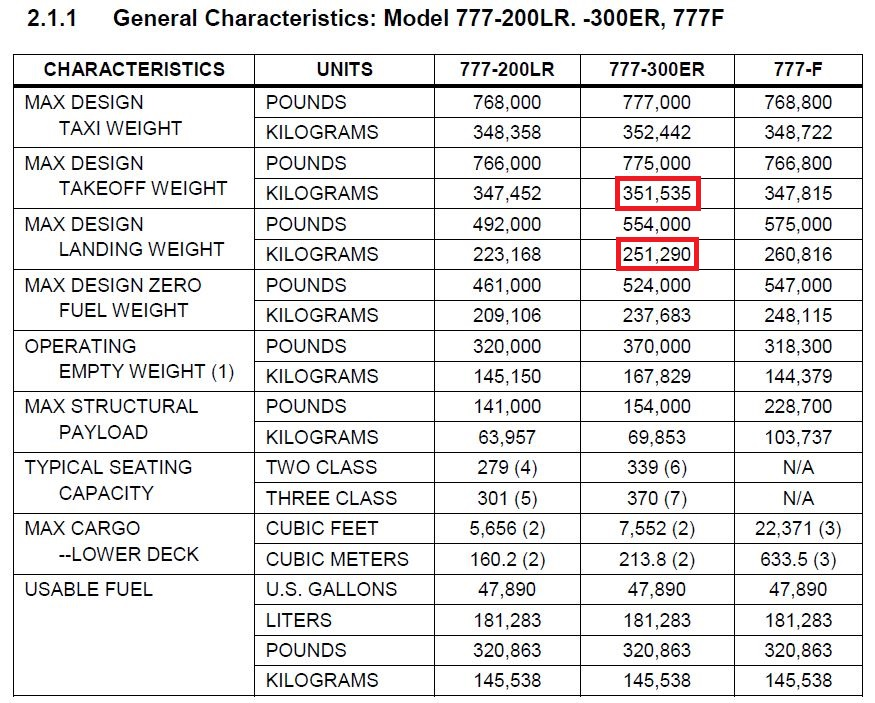
\includegraphics[clip, trim=0cm 0cm 0cm 0cm, width=1\textwidth]{./images/B777/B777MTOW}
				\caption{Maximum weights of the B777 depending on its configuration.} %nom de la figura
				\label{} %per denotar una referencia
			\end{figure}

			The next step is to calculate using the following graph the takeoff distance required with standard day + 15ºC = 30ºC and sea level conditions.
			
			\begin{figure}[H]
				\centering
				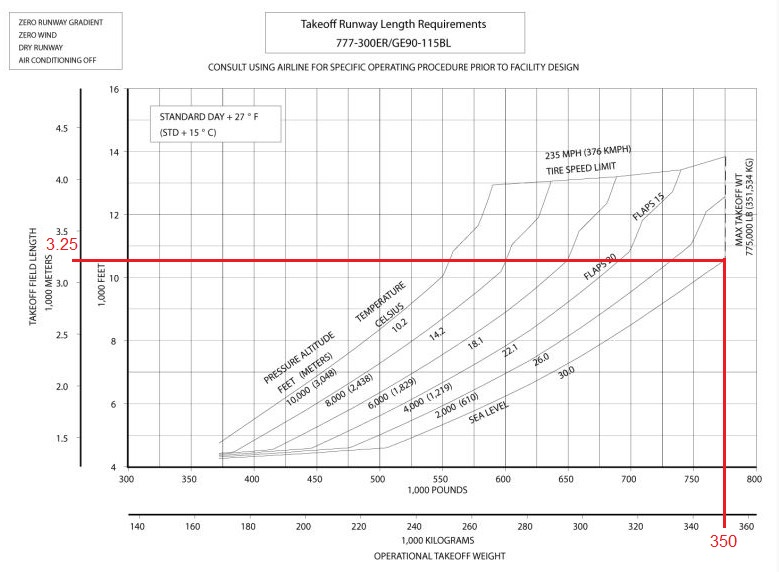
\includegraphics[clip, trim=0cm 0cm 0cm 0cm, width=1\textwidth]{./images/B777/payload-takeoffdistance}
				\caption{Relation between the MTOW and the takeoff distance.} %nom de la figura
				\label{} %per denotar una referencia
			\end{figure}
			
			As it is seen on the graph above, the length taken as reference (LCR) is 3.250m in a standard day+15ºC and sea level conditions. 
			
			The same procedure has to be done with the Airbus A330-300 in order to compare with one is the most restrictive one. Using the ACAP (Aircraft Characteristic for Airport Planning), the MTOW and MLW obtained are the following:
			
			\begin{figure}[H]
				\centering
				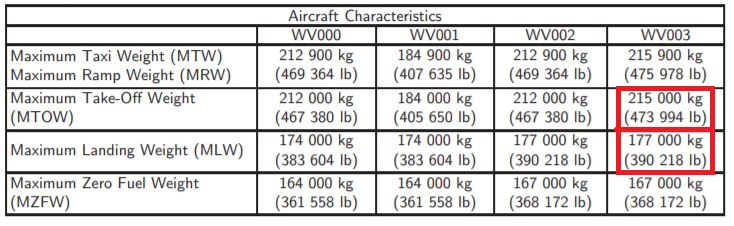
\includegraphics[clip, trim=0cm 0cm 0cm 0cm, width=1\textwidth]{./images/A330/A330}
				\caption{Maximum A330's weights.} %nom de la figura
				\label{} %per denotar una referencia
			\end{figure}
			
			Since the difference on the MTOW and MLW between both planes is greater than a 50\%, the Boeing’s Reference Field Length is chosen as the critical without calculating the Reference Field Length of the A330-300.
			
			Once the most restrictive plane is chosen, the next step is to correct the length following OACI’s instructions. The equation used to correct the altitude difference is:
			
			\[L_t=RFL*(1+0,07*\frac{\Delta h}{300})\]
			
			Solving the equation for a RFL of 3.250m and an increase on the altitude of 100m, the result obtained is 3326m.
			Since the temperature has already been corrected on the graph and the runway slope is going to be less than 0,5\% and thus, it can be neglected, the final length will be 3.500m rounding up.
		
			\subsubsection{Reference code}
			Using the dimensions of the B777-300ER and the tables given by the OACI, the number and letter that define the runway can be obtained. 
			
			\begin{figure}[H]
				\centering
				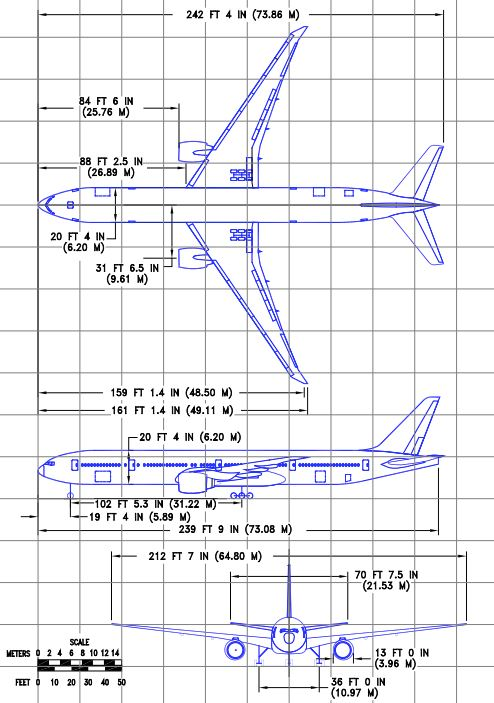
\includegraphics[clip, trim=0cm 0cm 0cm 0cm, width=1\textwidth]{./images/B777/Dimensions777}
				\caption{Boeing 777-300ER dimensions.} %nom de la figura
				\label{} %per denotar una referencia
			\end{figure}
				
			\begin{figure}[H]
				\centering
				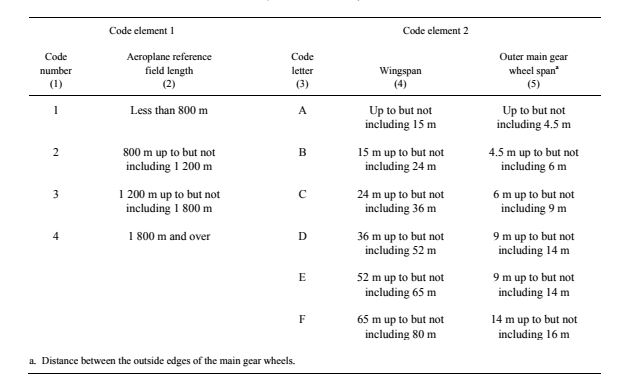
\includegraphics[clip, trim=0cm 0cm 0cm 0cm, width=1\textwidth]{./images/Annex14/Referencecode}
				\caption{Reference code given by the OACI.} %nom de la figura
				\label{} %per denotar una referencia
			\end{figure}
		
		\paragraph{}Due to the RFL being higher than 1800m , the reference number of the runway is number 4 according to OACI and due to the dimensions of the airplane B777-300ER, which has a span of 64,8m<65m and a distance between the landing gear of 10,97m<14m, the letter that defines the airport is E.
			
			\subsubsection{Runway width and shoulders}
			\paragraph{}The runway width is obtained using the OACI recommendations stated on the Annex 14 and the key reference of the runway. 
			
			\begin{figure}[H]
				\centering
				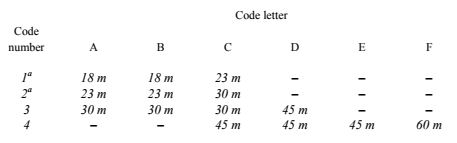
\includegraphics[clip, trim=0cm 0cm 0cm 0cm, width=1\textwidth]{./images/Annex14/RunwayWidth}
				\caption{Runway width according to OACI.} %nom de la figura
				\label{} %per denotar una referencia
			\end{figure}
		
			As it can be seen, and remembering that our key reference is 4E, the minimum runway width needed is 45m. This value has to be further increased with the use of runway shoulders up to a minimum of 60m. 

			\subsubsection{Declared distances}
			\paragraph{} The calculations done in order to obtain the final value can be seen on the airside’s attachments section 1. 
			
			To sum up, the final values obtained are:
			
			\subsubsection{Runway strips}
			\subsubsection{Runway end safety area (RESA)}
			\subsubsection{Stopway (SWY)}
			\subsubsection{Clearway (CWY)}
		